\section{Modified Valiant's algorithm}

In this section we describe the reorganization of submatrix processing order in the Valiant's algorithm which simplify independent handling of submatrices. As a result, proposed modification can facilitate implementation of parallel submatrix processing.

\subsection{New approach}

The main change of this modification is the possibility to divide the parsing table into layers of disjoint submatrices of the same size.
The idea of division we have made from the reorganization of the matrix multiplication order is presented in figure~\ref{fig3}.
Each layer consists of square matrices which size is power of 2.
The layers are computed successively in the bottom-up order.
Each matrix in the layer can be handled independently, which can help to implement parallel version of layer processing function.

\begin{figure}
    \centering
    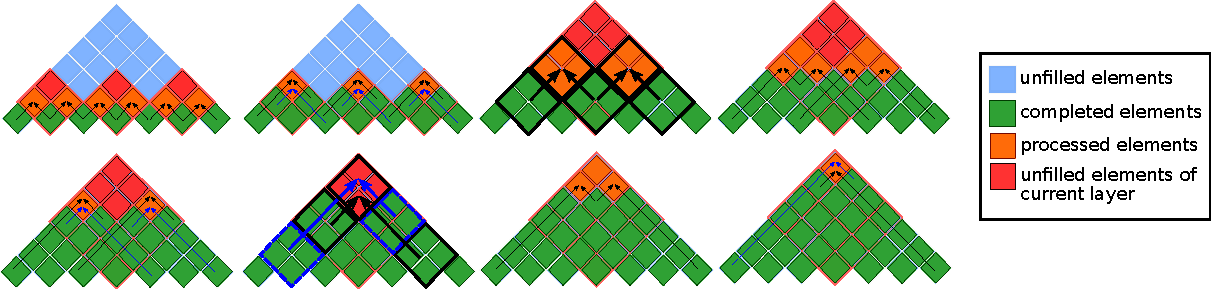
\includegraphics[width=0.9\textwidth]{pictures/modivis2.pdf}
    \caption{An example of the modification of Valiant's algorithm}
    \label{fig4}
\end{figure}

A simple example of the modification is shown in figure~\ref{fig4}. 
The lowest layer (submatrices which size is 1) is already computed and filling of the matrix starts with the second layer (????subfigures???? 1-2). 
Note that the same  process is presented in figure~\ref{fig1}, but here it can be done only in two steps using parallel computation of submatrix products.

The modified version of Valiant's algorithm is presented in listing~\ref{algo:modified}.
The procedure \textit{main()} computes the lowest layer $(T_{l, l+1})$, and then divide the table into layers, described earlier, and computes them through the \textit{completeVLayer()} call.
Thus, \textit{main()} computes all elements of parsing table $T$.
(Hereinafter, we use layer to mean set of submatrices.)

For brevity, we define \textit{left(subm), right(subm), top(subm), bottom(subm), rightgrounded(subm)} and \textit{leftgrounded(subm)} functions which returns the submatrices for matrix $subm = (l, m, l', m')$ according to the original Valiant's algorithm (figure~\ref{fig2}).

Also denote some subsidiary functions for matrix layer $M$:
 \begin{itemize}
  \item \textit{bottomsublayer(M)} $ = \{bottom(subm)\, |\,subm \in M \}$,
  \item \textit{leftsublayer(M)} $ = \{\textit{left(subm)}\, |\,subm \in M \}$,
  \item \textit{rightsublayer(M)} $ =\{\textit{right(subm)}\, |\,subm \in M \}$,
  \item \textit{topsublayer(M)} $ = \{top(subm)\, |\,subm \in M \}$.
\end{itemize}

\begin{algorithm}[h!]
\SetAlgoNoLine
\KwIn{$G = (\Sigma, N, R, S), w = a_{1} \dots a_{n}, n \geq 1, n + 1 = 2^p, a_{i} \in \Sigma$ }
\underline{main()}{:}{

 \For {$l \in \{1, \ldots, n \}$}{$T_{l, l + 1} = \{A | A \rightarrow a_{l + 1} \in R\}$}
 \For{$1 \le i < p - 1 $}{
 layer = \textit{constructLayer(i)}\;
 \textit{completeVLayer(layer)}
 }
 \BlankLine
 }

\underline{constructLayer(i)}{:}{
 \BlankLine
 $\{(k2^i, (k+1)2^i, (k + 1)2^i, (k+2)2^i) \, |\, 0 \le k < 2^{p - i} - 1\}$
 \BlankLine
    }
\underline{completeLayer(M)}{:}{
\BlankLine
\If {$\forall (l, m, l', m') \in M \quad (m - l = 1)$}{\For{$ (l, m, l', m') \in M$}{$T_{l, l'} = f(P_{l, l'})$\;}}
\Else{
\textit{completeLayer(bottomsublayer(M))}\;
\textit{completeVLayer(M)}
}
\BlankLine
}

\underline{comleteVLayer(M)}{:}{
 \BlankLine
 \textit{multiplicationTasks$_1$ = \linebreak 
    \{$left(subm)$, $leftgrounded(subm)$, $bottom(subm)\, |\,subm \in M \} \cup \linebreak  \{right(subm), bottom(subm), rightgrounded(subm)\, |\,subm \in M\}$\;}
 \BlankLine
 multiplicationTask$_2$ = $\{top(subm), leftgrounded(subm), right(subm)\, |\,subm \in M\}$\;
 \BlankLine
 multiplicationTask$_3$ = $\{top(subm), left(subm), rightgrounded\, |\,subm \in M\}$\;
 \BlankLine
 \textit{performMultiplications(multiplicationTask$_1$)}\;
 \textit{completeLayer(leftsublayer(M) $\cup$ rightsublayer(M))}\;
 \textit{performMultiplications(multiplicationTask$_2$)}\;
 \textit{performMultiplications(multiplicationTask$_3$)}\;
 \textit{completeLayer(topsublayer(M))}

 }
 \BlankLine

 \underline{performMultiplication(tasks)}{:}{\\
 \For{$ (m, m1, m2) \in \textit{tasks}$}{$P_{m} = P_{m} \cup (T_{m1} \times T_{m2})$\;}
 }

\caption{Parsing by matrix multiplication: Modified Version}
\label{algo:modified}
\end{algorithm}

The procedure \textit{completeVLayer(M)} takes an array of disjoint submatrices $M$ which represents a layer.
For each \textit{subm = (l, m, l', m') $\in M$} this procedure computes \textit{left(subm), right(subm), top(subm)}.
The procedure assumes that the elements of \textit{bottom(subm)} and $T_{i, j}$ for all $i$ and $j$ such that $l \leq i < j < m$ and $  l' \leq i < j < m'$ are already constructed.
Also it is assumed that the current value of
$P_{i, j} =  \{ (B, C) | \exists k, (m \le k < l'), a_{i + 1} \dots a_{k} \in L_G(B), a_{k + 1} \dots a_{j} \in L_G(C)\} $ for all $i$ and $j$ such that $l \leq i < m$ and $l' \leq j < m'$.

The procedure \textit{completeLayer(M)} also takes an array of disjoint submatrices $M$, but unlike the previous one, it computes $T_{i, j}$ for all $(i, j) \in subm$.
This procedure requires exactly same assumptions on $T_{i, j}$  and $P_{i, j}$  as in the previous case.

In the other words, \textit{completeVLayer(M)} computes the entire layer \textit{M} \linebreak and \textit{completeLayer($M_{2}$)} is a support function which is necessary for computation of smaller square submatrices $subm_{2} \in M_{2}$ inside of \textit{M}.  

Finally, the procedure \textit{performMultiplication(tasks)}, where \textit{tasks} is an array of a triple of submatrices, perform basic step of algorithm: matrix multiplication. It is worth mentioning that, as distinct from the original algorithm, here $|tasks| \ge 1$ and each task can be computed independently.
So, practical implementation of this procedure can easily involve different techniques of parallel array processing, such as OpenMP~\ref{!!!}.


\subsection{Correctness and complexity}

We provide the proof of correctness and time complexity for the proposed modification in this section.
To do it we should prove correctness of subprocedure \textit{completeLayer}.

\begin{lemma}
If the procedure \textit{completeLayer(M')} with start conditions:
\begin{enumerate}
  \item $T_{i, j} = \{ A |  a_{i + 1} \dots a_{j} \in L_G(A)\}$ for all $i$ and $j$ such that $l1 \leq i < j < m1$ and $l2 \leq i < j < m2$;
  \item $P_{i, j} =  \{ (B, C) |\exists k, (m1 \le k < l2): a_{i + 1} \dots a_{k} \in L_G(B), a_{k + 1} \dots a_{j} \in L_G(C)\}$ for all $l1 \leq i < m1$ and $l2 \leq j < m2$.
\end{enumerate}
returns correctly computed sets of $T_{i, j}$ for all $l1 \leq i \le m1$ and $l2 \leq j \le m2$ for all $(l1, m1, l2, m2) \in M'$ for any layer $M'$ 
and for layer $M$ fulfilled that: 
\begin{enumerate}
  \item $T_{i, j} = \{ A |  a_{i + 1} \dots a_{j} \in L_G(A)\}$ for all $i$ and $j$ such that $l \leq i < j < m$ and $l' \leq i < j < m'$ and for $(i, j) \in bottom(M)$;
  \item $P_{i, j} =  \{ (B, C) |\exists k, (m \le k < l'): a_{i + 1} \dots a_{k} \in L_G(B), a_{k + 1} \dots a_{j} \in L_G(C)\}$ for all $l \leq i < m$ and $l' \leq j < m'$.
\end{enumerate}

Then the procedure \textit{completeVLayer(M)} returns correctly computed sets of $T_{i, j}$ for all $l \leq i \le m$ and $l' \leq j \le m'$ for all $(l, m, l', m') \in M$. 
\end{lemma}

\begin{proof}

Firstly, \textit{performMultiplications(multiplicationTask$_1$)} adds to each P$_{i,j}$ all pairs 
$(B, C)$ such that $\exists k$, $(\frac{l+m}{2} \le k < l')$, $a_{i + 1} \dots a_{k} \in L_{G}(B)$, $a_{k + 1} \dots a_{j} \in L_{G}(C)$ for all $(i, j)$ $\in leftsublayer(M)$
and
$(B, C)$ such that $\exists k$, $(m \le k < \frac{l'+m'}{2})$, $a_{i + 1} \dots a_{k} \in L_{G}(B)$, $a_{k + 1} \dots a_{j} \in L_{G}(C)$ for all $(i, j)$ $\in rightsublayer(M)$.
Now \textit{completeLayer(leftsublayer(M) $\cup$ rightsublayer(M))} can be called and it returns correctly computed \textit{leftsublayer(M) $\cup$ rightsublayer(M)}.

Then \textit{performMultiplications} called with arguments 
\textit{multiplicationTask$_2$} and \textit{multiplicationTask$_3$} adds pairs 
$(B, C)$ such that $\exists k$, $(\frac{l+m}{2} \le k < m)$, $a_{i + 1} \dots a_{k} \in L_{G}(B)$, $a_{k + 1} \dots a_{j} \in L_{G}(C)$ 
and 
$(B, C)$ such that $\exists k$, $(l' \le k < \frac{l'+m'}{2})$, $a_{i + 1} \dots a_{k} \in L_{G}(B)$, $a_{k + 1} \dots a_{j} \in L_{G}(C)$
to each P$_{i,j}$ for all $(i, j)$ $\in topsublayer(M)$. 
So as $m = l'$ (from the construction of the layer), condition for elements of matrix $P$ are fulfilled.
Now \textit{completeLayer(topsublayer(M))} can be called and it returns correctly computed \textit{topsublayer(M)}.

Thus, all $T[i, j]$ $\forall (i, j) \in M$ are computed correctly.

\end{proof}

\begin{theorem}
Let $M$ be a layer. If for all $(l, m, l', m') \in M$:
\begin{enumerate}
  \item $T_{i, j} = \{ A |  a_{i + 1} \dots a_{j} \in L_G(A)\}$ for all $i$ and $j$ such that $l \leq i < j < m$ and $l' \leq i < j < m'$;
  \item $P_{i, j} =  \{ (B, C) |\exists k, (m \le k < l'): a_{i + 1} \dots a_{k} \in L_G(B), a_{k + 1} \dots a_{j} \in L_G(C)\}$ for all $l \leq i < m$ and $l' \leq j < m'$.
\end{enumerate}

Then the procedure \textit{completeLayer(M)}, returns correctly computed sets of $T_{i, j}$ for all $l \leq i \le m$ and $l' \leq j \le m'$ for all $(l, m, l', m') \in M$.
\end{theorem}


\begin{proof}(Proof by induction on $m - l$.)

Let $(l, m, l', m')$ be a typical element of array $M$.
As far as each element can be handled independently, we prove statements only for one element of $M$.

\underline{\textbf{Basis:}} $m - l = 1$. There is only one element to compute, and $P_{l, l'} =  \{ (B, C) |  a_{l + 1} \dots a_{l'} \in L(B)L(C)\}$. Further, algorithm computes $f(P[l, l'])$ = \linebreak $\{ A |  a_{l + 1} \dots a_{l'} \in L(A)\}$, so $T[l, l']$ computed correctly.

\underline{\textbf{Inductive step:}} Assume that $(l_1, m_1, l_2, m_2)$ is correctly computed for all $m_2 - l_2 = m_1 - l_1 < m - l$.

Consider \textit{completeLayer(M)} call, where $m - l > 1$.

Firstly, consider \textit{completeLayer(bottomsublayer(M))}.
Theorem conditions are fulfilled, then this call returns correct sets $T_{i, j}$ for all $(i, j) \in bottomsublayer(M)$. It should be noted that the theorem conditions allow $T_{m, l'}$ (the lowest element) be correctly computed as in base case.

As \textit{bottomsublayer(M)} now calculated,\textit{completeVLayer(M)} can be called.

All $T_{i,j}$ are already calculated for all $i$ and $j$ such that $l \leq i < j < m$ and $l' \leq i < j < m'$, because of the theorem conditions.  All lemma 1 conditions are fulfilled and all $T[i, j]$ $\forall (i, j) \in M$ are computed correctly.
\end{proof}

\begin{theorem}
Algorithm from listing~\ref{algo:modified} correctly computes $T_{i, j}$ for all i and j, thus an input string $a = a_{1}a_{2} \dots a_{n} \in L_{G}(S)$ if and only if $S \in T_{0, n}$.
\end{theorem}

\begin{proof}

Primarily to prove the theorem, we show by induction that all layers of the parsing table T are computed correctly.

\underline{\textbf{Basis:}} layer of size $1 \times 1$.
Parsing table \textit{T} consists of one layer of size 1 and its elements are correctly computed in lines 2-3 in listing~\ref{algo:modified}.

\underline{\textbf{Inductive step:}} assume any layer of size less than or equal to $2^{p - 2} \times 2^{p - 2}$ are computed correctly. 

Define layer of size $2^{p - 1} \times 2^{p - 1}$ as M. 
Hereinafter \textit{subm = (l, m, l', m')} is a typical element of layer M.

Consider \textit{completeVLayer(M)} call. 

All $T_{i,j}$ are already calculated for all $i$ and $j$ such that $l \leq i < j < m$ and $l' \leq i < j < m'$, because these elements lie in layers which are already computed.

All lemma 1 and theorem 1 conditions are fulfilled. Thus, \textit{completeVLayer(M)} returns correct $T_{i, j}$ for all $(i, j)$ $\in M$ for any layer M of parsing table T and lines 4-6 in listing~\ref{algo:modified} return all $T_{i, j} =  \{ A | A \in N, a_{i + 1} \dots a_{j} \in L_{G}(A)\}$.

\end{proof}

\begin{lemma}
Let \textit{calls$_{i}$} is a number of the calls of \textit{completeVLayer(M)} where for all $(l, m, l', m') \in M$ with $m - l = 2^{p - i}$.
\begin{itemize}
 \item for all $i \in \{ 1, .., p - 1\}$  $\sum_{n=1}^{calls_i}{|M|}$ is exactly $2^{2i - 1} - 2^{i - 1}$;
 \item for all $ i \in \{ 1, .., p - 1\}$ products of submatrices of size $2^{p - i} \times 2^{p - i}$ are calculated exactly $2^{2i - 1} - 2^{i}$ times.
\end{itemize}
\end{lemma}

\begin{proof}

Prove the first statement by induction on i.

\underline{\textbf{Basis:}} i = 1. \textit{calls$_{1}$} and $|M| = 1$. So, $2^{2i - 1} - 2^{i - 1} = 2^1 - 2^0 = 1$.

\underline{\textbf{Inductive step:}} assume that $\sum_{n=1}^{calls_i}{|M|}$ is exactly $2^{2i - 1} - 2^{i - 1}$ for all $i \in \{ 1, .., j\}$.

Let us consider $i = j + 1$.

Firstly, note that function $\textit{costructLayer(i)}$ returns $2^{p - i} - 1$ matrices of size $2^i$, so in the call of \textit{completeVLayer(costructLayer(k - i))}  \textit{costructLayer(k - i)} returns $2^i - 1$ matrices of size $2^{p - i}$. 
Secondly, \textit{completeVLayer(M)} is called 3 times for the left, right and top submatrices of size $2^{p - (i - 1)}$. Finally, \textit{completeVLayer(M)} is called 4 times for the bottom, left, right and top submatrices of size $2^{p - (i - 2)}$, except $2^{i - 2} - 1$ matrices which were already computed.

Then, $\sum_{n=1}^{calls_i}{|M|} = 2^{i} - 1 + 3 \times (2^{2(i - 1) - 1} - 2^{(i - 1) - 1}) + 4 \times (2^{2(i - 2) - 1} - 2^{(i - 2) - 1}) - (2^{i - 2} - 1) = 2^{2i - 1} - 2^{i - 1}$.

Now we know that $\sum_{n=1}^{calls_{i-1}}{|M|}$  is $2^{2(i - 1) - 1} - 2^{(i - 1) - 1}$ and we can calculate the number of products of submatrices of size $2^{p - i} \times 2^{p - i}$. 
During these calls \textit{performMultiplications} run 3 times, $|multiplicationTask1| = 2 \times 2^{2(i - 1) - 1} - 2^{(i - 1) - 1}$ and $|multiplicationTask2|$ = $|multiplicationTask3| = 2^{2(i - 1) - 1} - 2^{(i - 1) - 1}$. So, the number of products of submatrices of size $2^{p - i} \times 2^{p - i}$ is $ 4 \times (2^{2(i - 1) - 1} - 2^{(i - 1) - 1}) = 2^{2i - 1} - 2^{i}$.
\end{proof}

\begin{theorem}
Let $|G|$ be a length of the description of the grammar G and let n be a length of an input string. Then algorithm from listing~\ref{algo:modified} calculates matrix \textit{T} in $\mathcal{O}(|G|BMM(n)\log{n})$ where BMM(n) is the number of operations needed to multiply two Boolean matrices of size $n \times n$.
\end{theorem}

\begin{proof}
The proof is almost identical with that of the theorem given by Okhotin~\cite{Okhotin:2014:PMM:2565359.2565379}, because, as shown in the last lemma, the Algorithm 1 has the same number of products of submatrices.
\end{proof}

To summarize, the correctness of the modification was proved and it was shown that the time complexity remained the same as in Valiant's version.

\subsection{Algorithm for substrings}

Next we show how our modification can be applied to the string-matching problem.

So if we want to find all substrings of size $s$ which can be derived from a start symbol for an input string of size $n = 2^p$, we need to compute layers with submatrices of size not greater than $2^{l'}$, where $2^{l' - 2} < s \le 2^{l' - 1}$.

Let $l' = p - (m - 2)$ and consequently $(m - 2) = p - l'$.

For any  $m \le i \le p$ products of submatrices of size $2^{p - i}$ are calculated exactly $2^{2i - 1} - 2^{i}$ times and each of them imply multiplying $\mathcal{O}(|G|)$ Boolean submatrices.

$ C \sum\limits_{i=m}^p 2^{2i - 1} \cdot 2^{\omega(p - i)} \cdot f(2^{p - i}) = C \cdot 2^{\omega l'}\sum\limits_{i=2}^{l'} 2^{(2 - \omega)i} \cdot 2^{2(p - l') - 1} \cdot f(2^{l' - i}) \le C \cdot 2^{\omega l'} f(2^{l'}) \cdot 2^{2(p - l') - 1} \sum\limits_{i=2}^{l'} 2^{(2 - \omega)i} = BMM(2^{l'}) \cdot 2^{2(p - l') - 1} \sum\limits_{i=2}^{l'} 2^{(2 - \omega)i}$

Thus, time complexity for searching all substrings is  $O(|G|BMM(2^{l'})(l' - 1))$, while time complexity for the full input string is $O(|G|BMM(2^p)(p - 1))$. In contract to the modification, Valiant's algorithm completely calculate at least 2 triangle submatrices of size $\frac{n}{2}$ (as shown in figure~\ref{fig5}) which mean minimum asymptotic complexity  $O(|G|BMM(2^{p - 1})(p - 2))$. Make a conclusion that the modification is asymptotically faster for substrings of size $s \ll n$  than the original algorithm.

\begin{figure}
    \centering
    \captionsetup{justification=centering}
    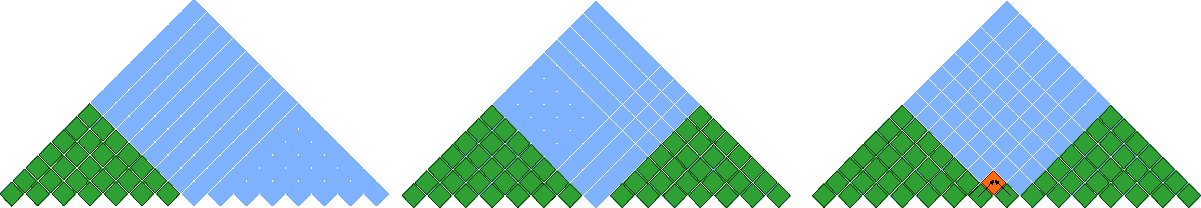
\includegraphics[width=0.9\textwidth]{pictures/valsubstring.pdf}
    \caption{The number of elements necessary to compute in Valiant's algorithm. That means it is nessesary to calculate at least 2 triangle submatrices of size $\frac{n}{2}$.}
    \label{fig5}
\end{figure}
